\documentclass[11pt,a4paper]{report}
\usepackage[utf8]{inputenc}
\usepackage{amsmath}
\usepackage{amsfonts}
\usepackage{amssymb}
\usepackage[utf8]{inputenc}
\usepackage[T1]{fontenc}
\usepackage{textcomp}
\usepackage{gensymb}
\usepackage{graphicx}
\begin{document}


\section{Analyzing the scattering distribution}

In order to find an importance sampling function, the scattering distribution should be analyzed carefully. The importance sampling function should prefer to sample directions that contribute more to the rendering result than directions that hardly contribute. In this section we will look at several scattering distributions to understand how light spreads as it scatters through a fiber and/or multiple fibers.

\subsection{Scattering Distribution from Fixed Light Source}

Consider holding the light at a fixed incident direction $\omega_i$. The images in figure~\ref{visual_light_distribution} show the scattering distribution for hair fibers from a directional light source. The left images correspond to direct scattering, where light rays impinge directly on the hair fibers, without scattering through other fibers first. The images to the right show the indirect scattering response. Here light is scattered through one other fiber first, causing a spread in the distribution.

\begin{figure}[h]
\begin{tabular}{c}
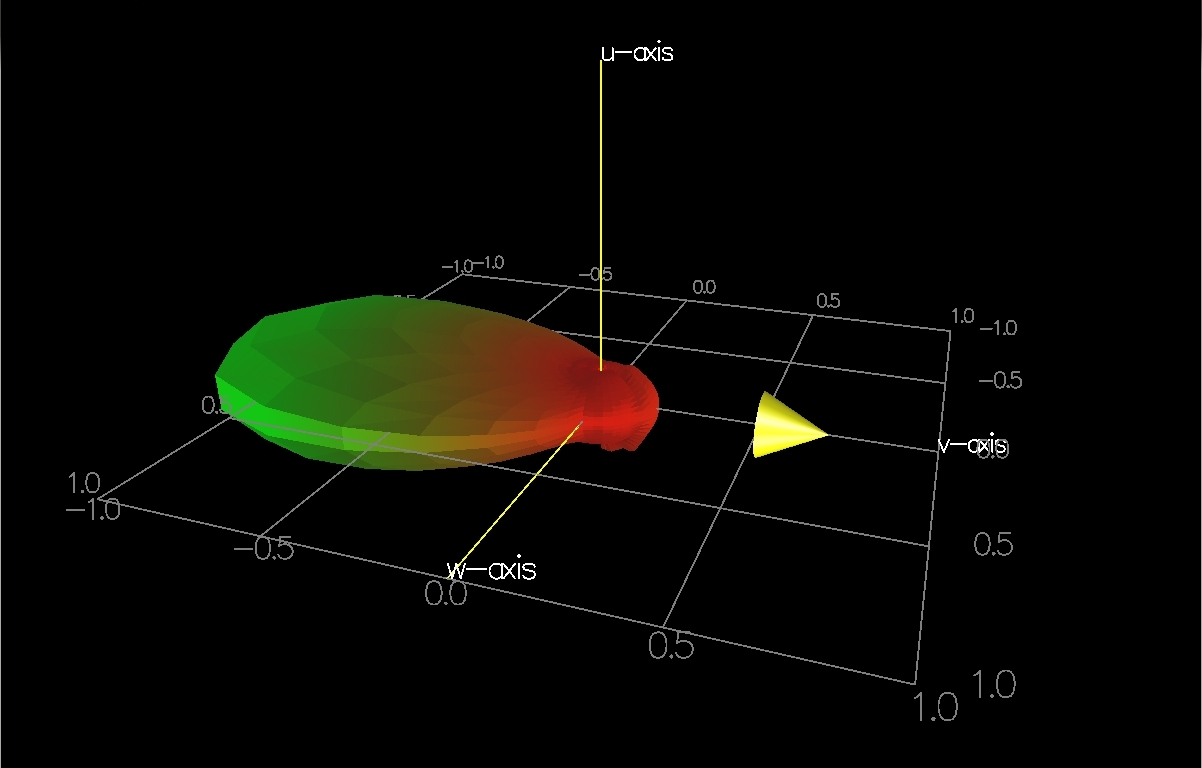
\includegraphics[scale=0.2]{images/strands0_colorR.jpg}
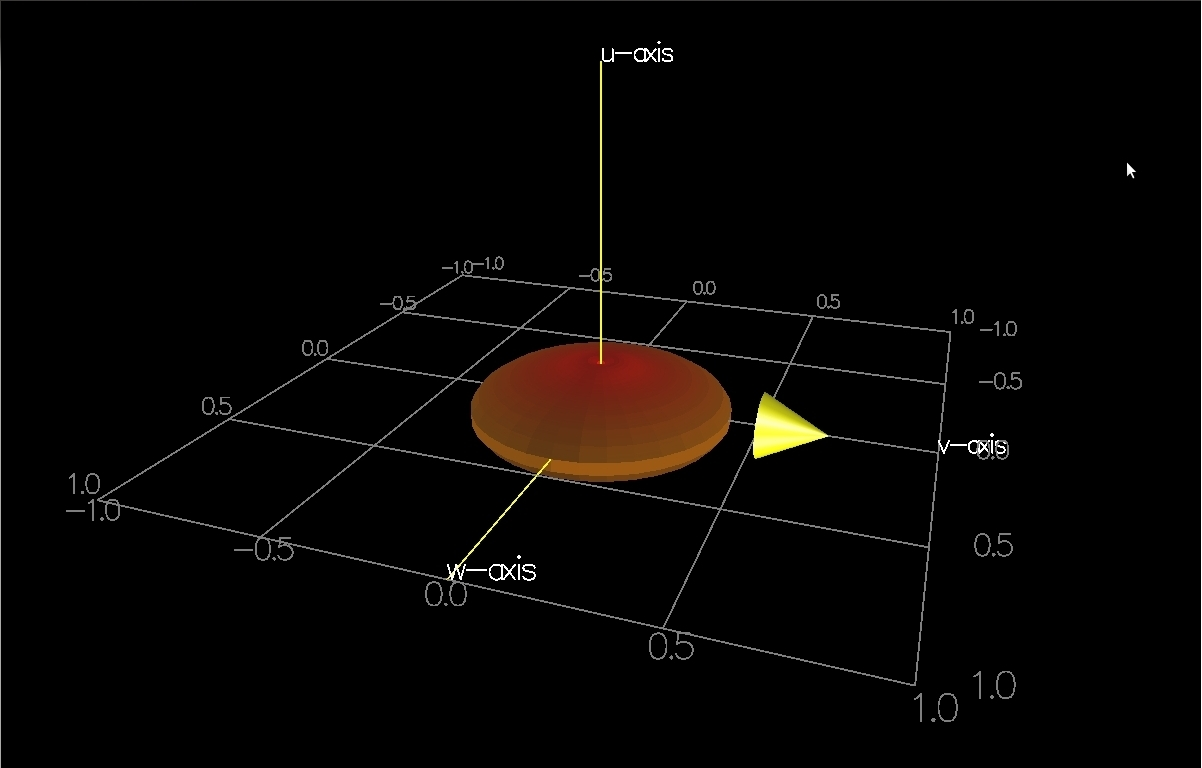
\includegraphics[scale=0.2]{images/strands1_colorR.jpg} \\
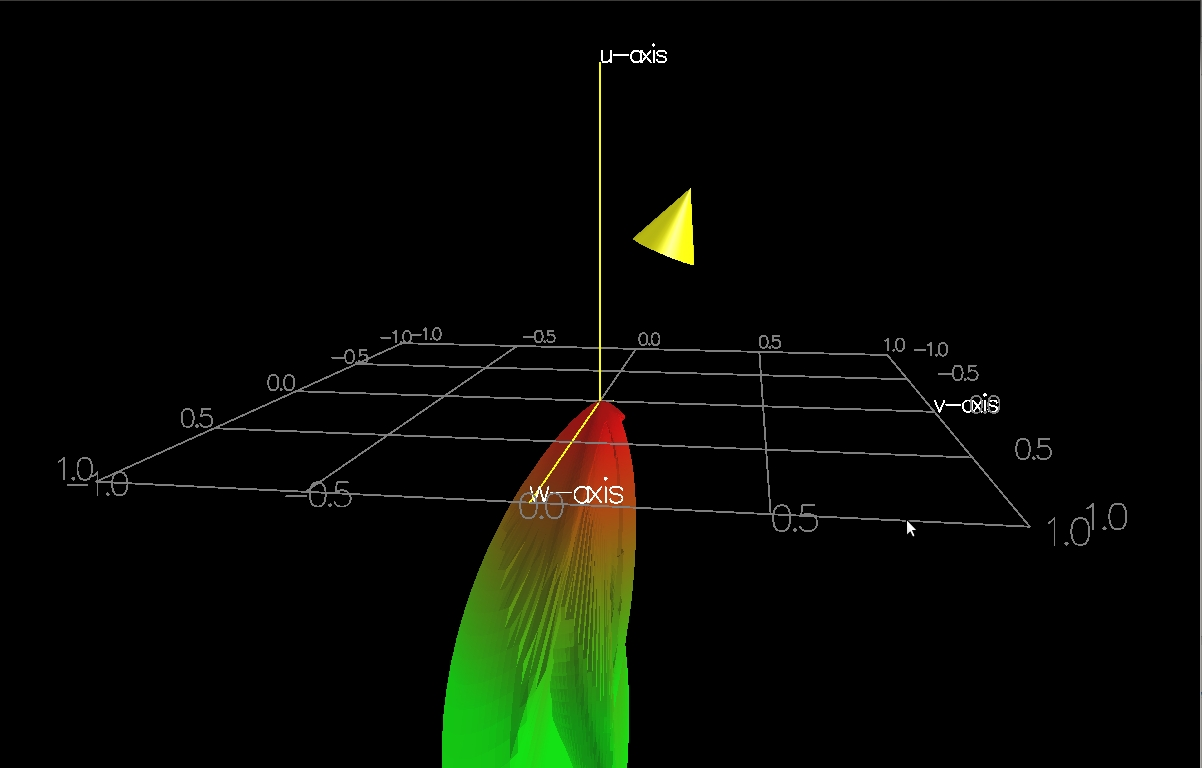
\includegraphics[scale=0.2]{images/theta67_strands0_colorR.jpeg}
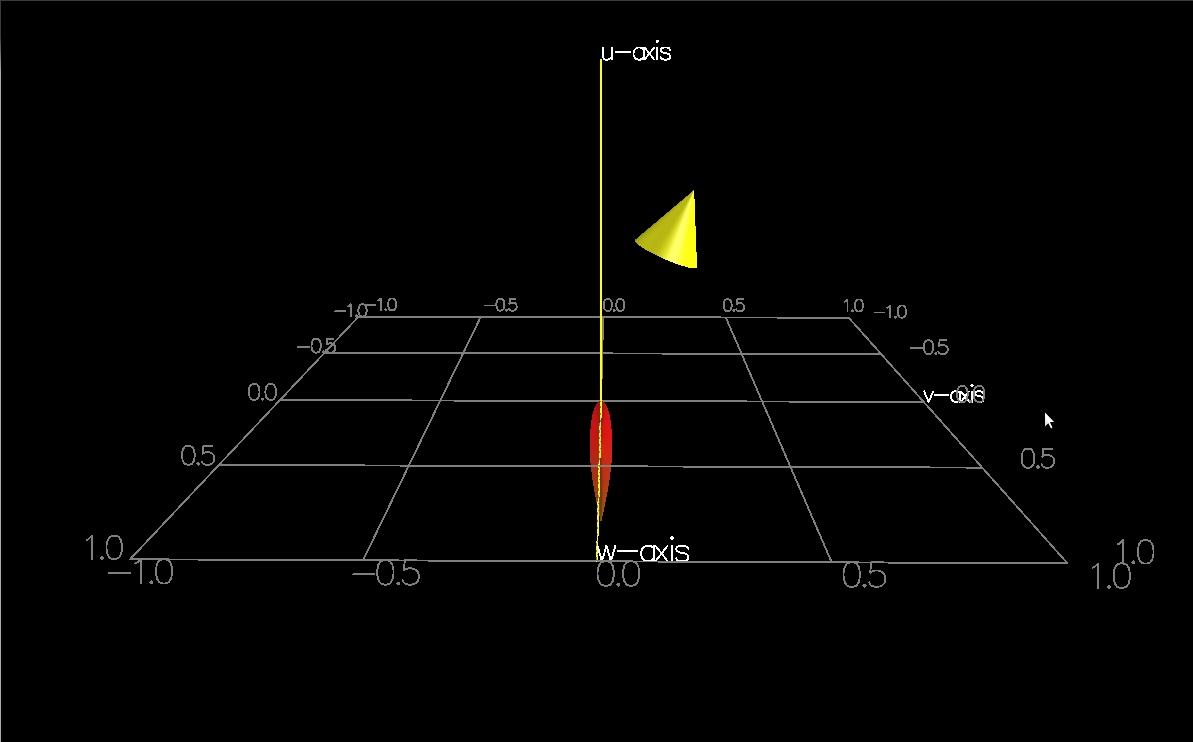
\includegraphics[scale=0.2]{images/theta67_strands1_colorR.jpeg} \\
\end{tabular}

\caption{Distribution of light when scattered against a hair fiber. The hair fiber runs along the u-axis and light is coming from the light source, depicted as the yellow cone. Images to the left show direct scattering. Images to the right show indirect scattering after 1 scattering event.}
\label{visual_light_distribution}

\end{figure}

Hair fibers that are directly hit by the light rays show a strong transmission component. This is what we expect, because Marschner et al.~\ref{marschner} did research to single fiber scattering and discovered that the transmission component is the most dominant component in giving the hair its color.

The scattering response for fibers that are indirectly hit show a more scattered distribution. After only one scattering event, the distribution becomes almost uniform in the azimuthal direction, but for the longitudinal direction, there is still a dependency in the longitudinal angles.

\subsection{Scattering Distribution for viewer direction versus incident light direction}

Rendering a globally illuminated scene is done using Monte-Carlo sampling. Monte-Carlo sampling uses a combination of two BRDFs: one for the light source and one for the material. It is important to use the BRDF for the light source in order to know which directions are affected by the light source and which directions are hardly lit. The same holds for the BRDF of the hair volume. It is this combination that makes rendering efficient. For importance sampling we need to sample directions according to the relative significance of sampling directions. We know the direction of the viewer $\omega_r$ and need to sample an incident light direction $\omega_i$. To do this we need to plot another scattering distribution that shows the response for any incident light direction $\omega_i$, given the direction of the viewer $\omega_r$.















A clear observation the can be made from the graphs, is that after only a single scattering event, the dependency on $\omega_i$ is almost completely negligible. The dependence on $theta_i$ is still present, but decreases after more scattering events eventually becoming a uniform distribution as well. The reason that this is obvious is because the model makes a distinction based on whether the point to be shaded is directly lit or indirectly lit.

So, we can separate the distributions based on having a single-scattering scenario, or a multiple scattering scenario.


So we can view the graphs as single scattering (comparative to the Marschner model) and the multiple scattering scenario 


Importance sampling is quite challenging in this case, since we are not only dealing with a complex scattering distribution, that we want to importance sample. We are also dealing with an unusual setting, namely that the scattering behaviour is dependent on the location inside the hair volume: points on the edge of the model are directly lit from one hemisphere, but also indirectly lit from the other side of the hemisphere.

















\section{Constructing the importance sampling function}



\begin{figure}[h]
\begin{center}
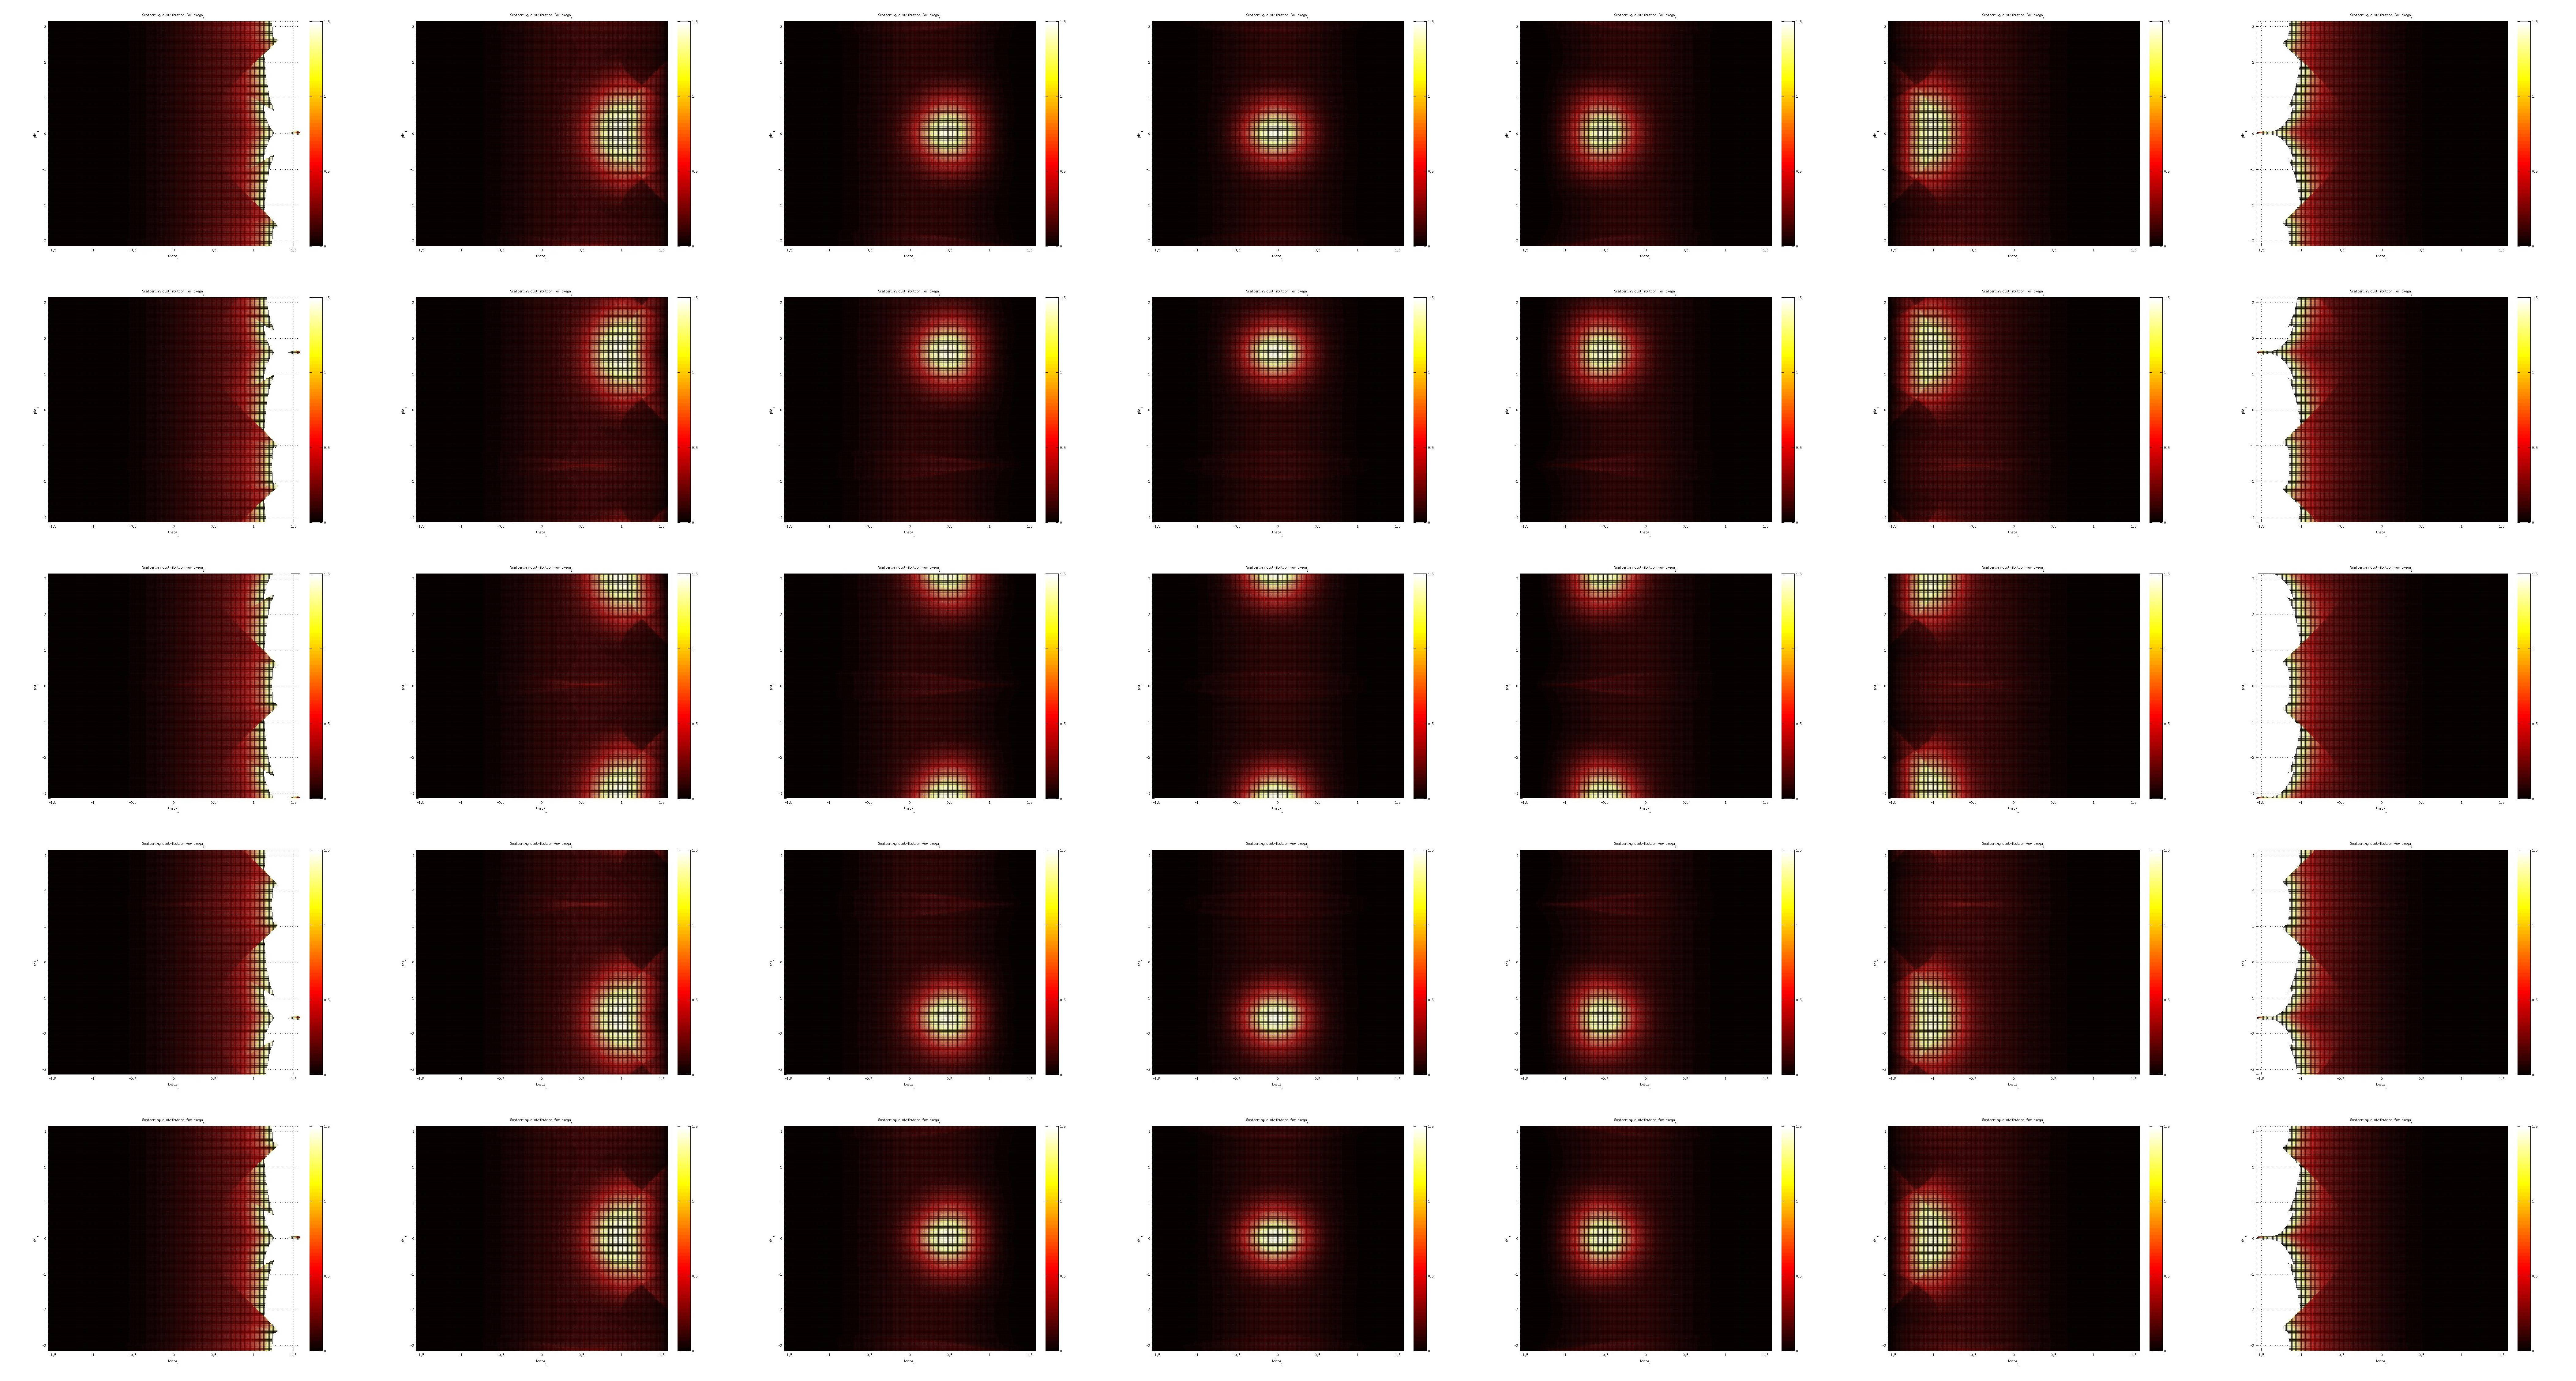
\includegraphics[scale=0.04]{images/scatteringdistribution/numstrands0.jpg}
\caption{The scattering distribution when no hair strands are between the viewer and the shading point (direct scattering). Each graph represent a different setting for $\omega_r = (\theta_r, \phi_r)$. Going from left to right (7 graphs), the value of $\theta_r$ is -90, -60, -30, 0, 30, 60 and 90 degrees. Going from top to bottom (5 graphs), the value of $\phi_r$ is 180, 90, 0, -90 and -180 degrees. Each of the smaller graphs represent variations in $\omega_i = (\theta_i, \phi_i)$. In this way, the collection of graphs show what incident light directions have a strong contribution for different directions of the viewer $\omega_r$.}
\label{numstrands0}
\end{center}
\end{figure}

\begin{figure}[h]
\begin{center}
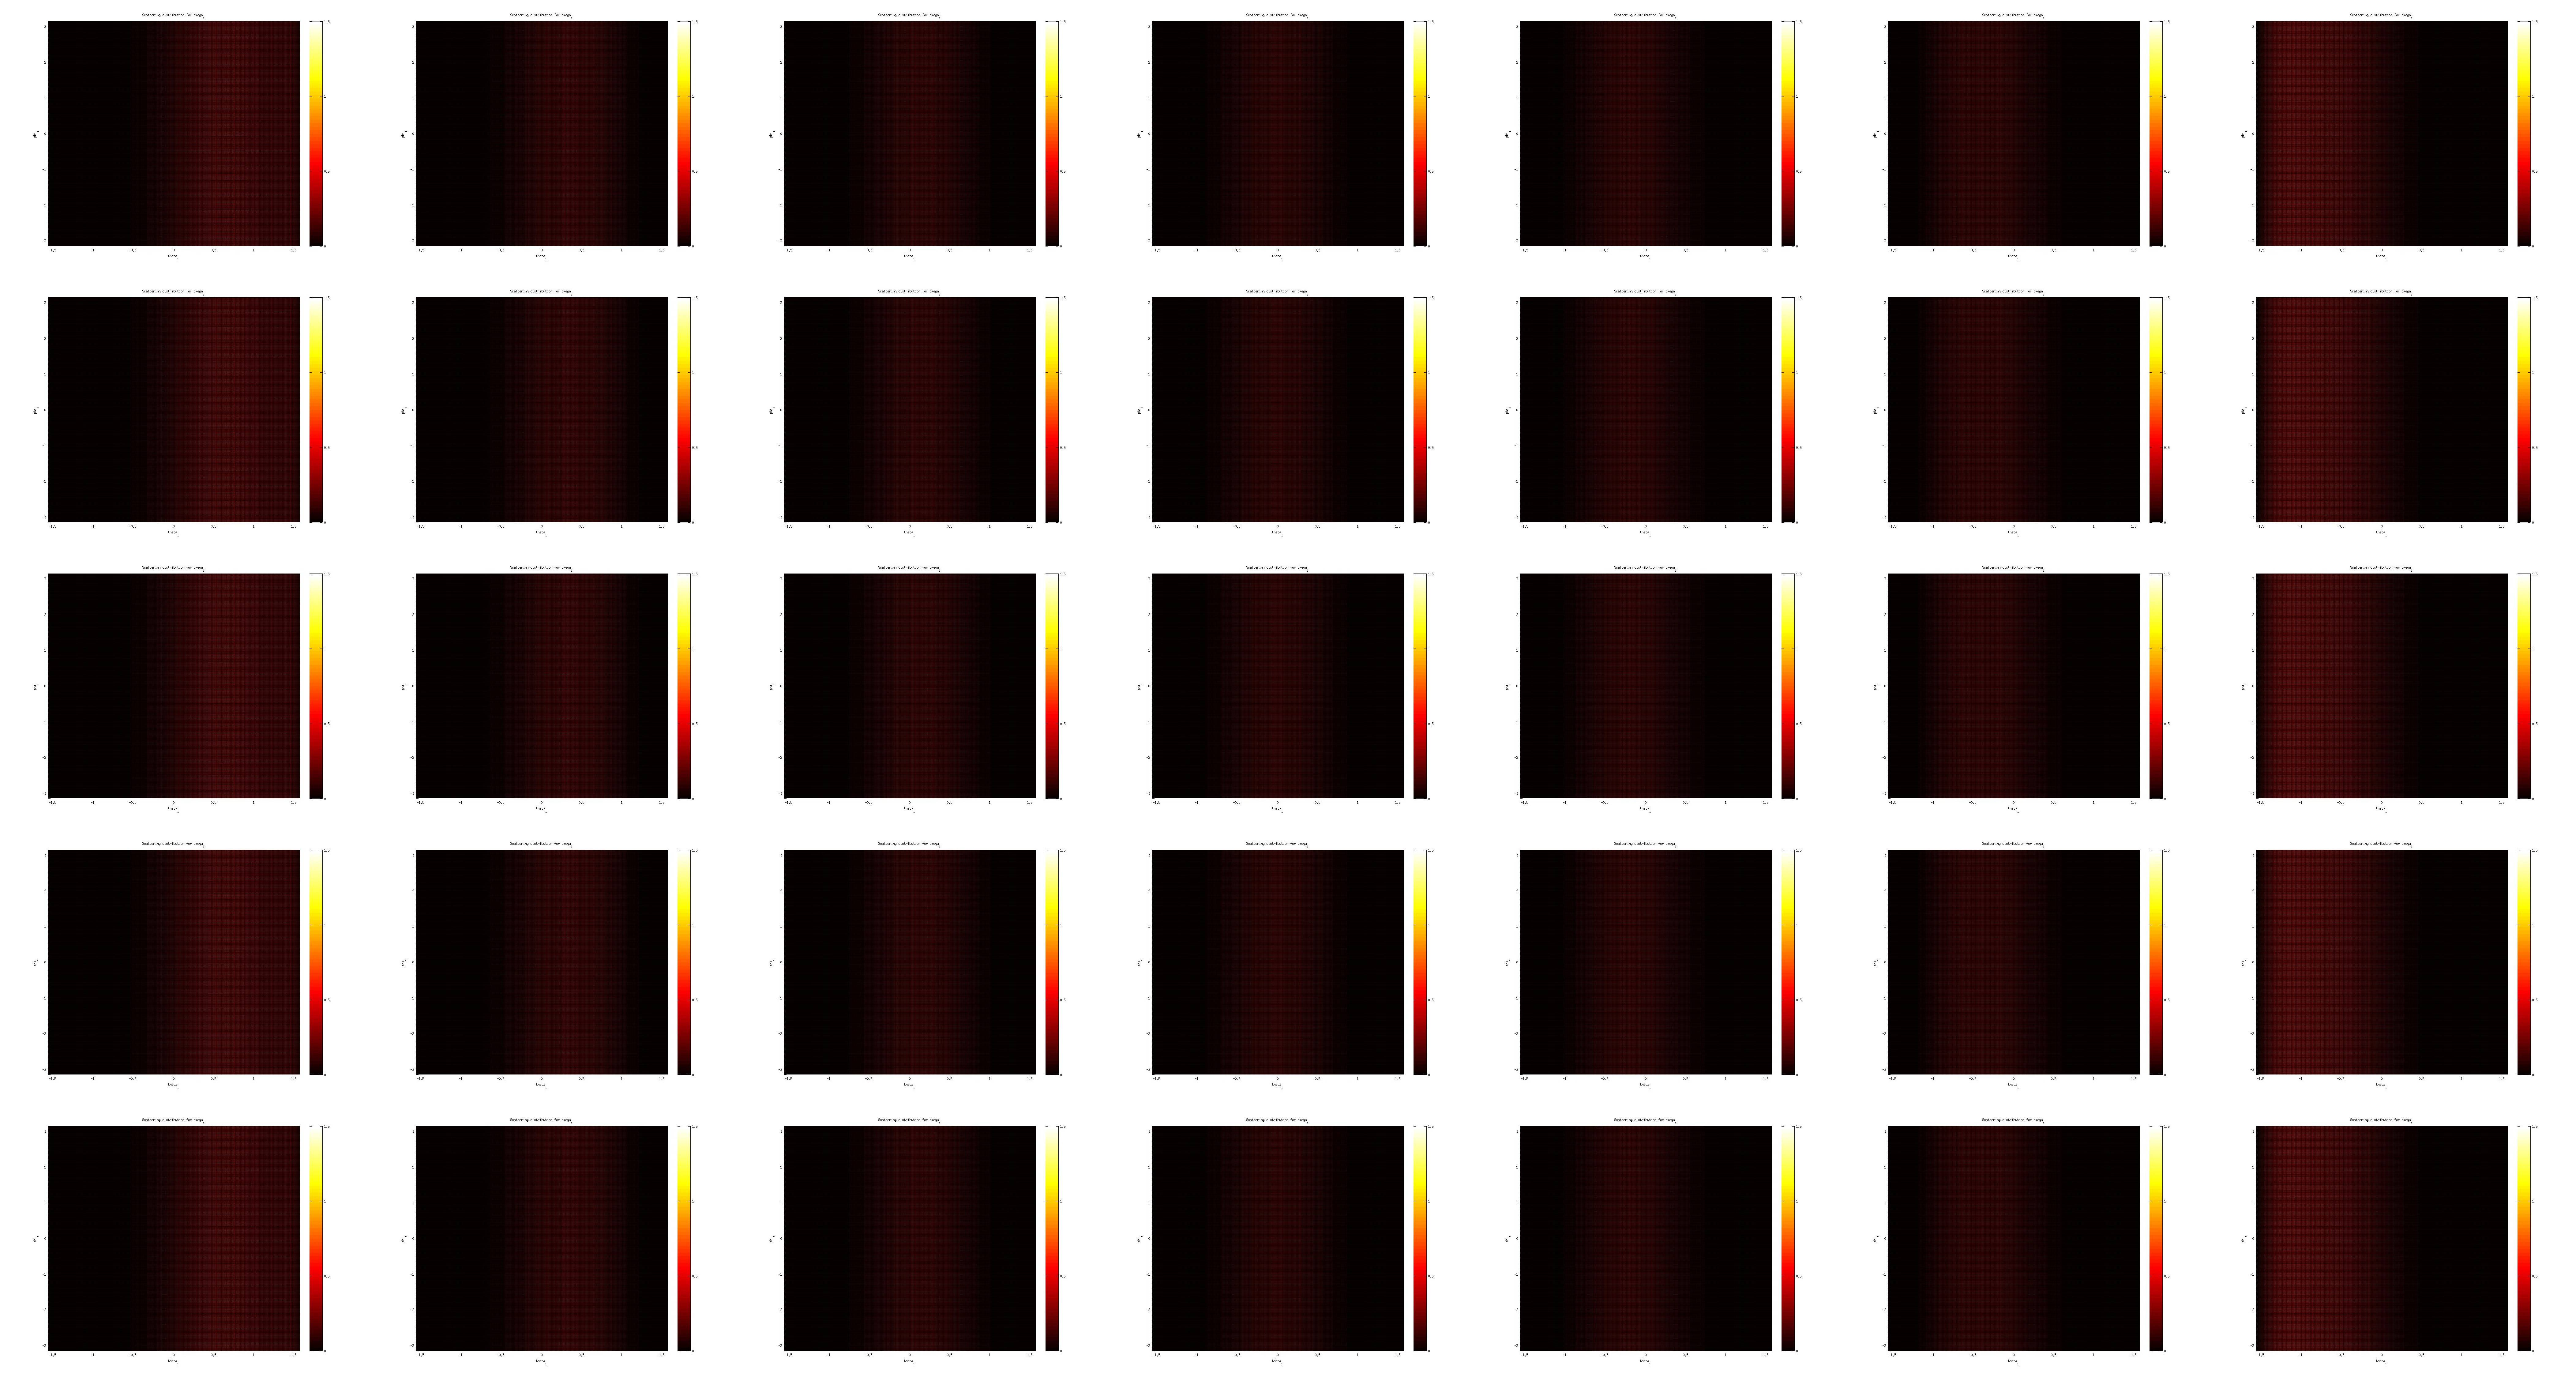
\includegraphics[scale=0.04]{images/scatteringdistribution/numstrands2.jpg}
\caption{Similarly to figure~\ref{numstrands0}, this graph depicts the same information but now for two hair strands (indirect scattering).}
\label{numstrands2}
\end{center}
\end{figure}

The scattering distribution shows which incident light directions $\omega_i$ are preferred to be sampled for a given viewer direction $\omega_r$. To be able to sample a direction, three steps should be performed. 

\begin{enumerate}
\item A probability density function (PDF) should be created that accurately matches the scattering distribution.
\item The PDF needs to be integrated to a normalized cumulative distribution function (CDF).
\item The CDF needs to be inverted to an inverted CDF.
\end{enumerate}

In this section, the creation of the PDF is explained. The PDF should  accurately match the scattering distribution. The more accurate it matches the distribution, the better the sampling will become. Since the scattering distribution differs between directly illuminated strands, versus indirectly illuminated strands, a choice is made to create two different probability density functions that are combined together. These are the direct scattering PDF and the multiple scattering PDF.



 The direct scattering is more complex to be matched. 

\subsubsection{Fitting the direct scattering distribution}

The direct scattering distribution is a bit trickier to fit, because of the dependency on both $\theta_r$ and $\phi_r$. We want to approximate the elliptical highlight, clearly visible in the scattering distribution (figure~\ref{numstrands0}). The idea is to break down the probability density function into two Gaussian functions: one for the variation in the longitudinal direction ($\theta_i$) and one for the azimuthal variation ($\phi_i$). The Gaussian functions can then be fitted separately for each direction and combined by multiplication to form the approximation of the scattering distribution.

As the light rotates around the hair fiber, so does the highlight rotate around the fiber. It turns out that the highlight is always opposite to the incident azimuthal direction $\phi_i$. Assuming that the azimuthal component of the incident light direction $\phi_i = x\degree$, then the highlight will always be observed at $\phi_r = x+180\degree$. This means that we can combine 
[TODO: Propose general function]



Figure~\ref{numstrands0} shows that as the viewer moves around the hair fiber, then the highlight rotates around it as well, but the shape remains the same. Using this knowledge, the PDF becomes much simpler to construct. That means that we only need to look at the difference to the gaussian functions when varying $\theta_r$. A change of $\phi_r$ will thus have no impact on the shape of the gaussians.

To fit the function we consider the center point $(\theta_i^C, \phi_i^C)$ of the elliptical highlight. Instead of choosing the center point of the highlight manually, we choose the center point by finding the maximum value of the distribution. The table below shows the maximum values and their corresponding incident light direction $\omega_i$.

\begin{table}
\begin{center}
\begin{tabular}{c||c|c|c|c|c|c|c|}

$\phi_i$ / $\theta_i$ & $-90\degree$ & $-60\degree$ & $-30\degree$ & $0\degree$ & $30\degree$ & $60\degree$ & $90\degree$ \\ \hline \hline
$-180\degree$ & $(90\degree, -178\degree)$  & $(56\degree, -14\degree)$ & $(27\degree, -3\degree)$ & $(-2\degree, -1\degree)$ & $(-31\degree, -3\degree)$ & $(-59\degree, -15\degree)$ & $(-89\degree, -176\degree)$ \\ \hline
$-90\degree$ & $(90\degree, -91\degree)$ & $(56\degree, 104\degree)$ & $(27\degree, 90\degree)$ & $(-2\degree, 90\degree)$ & $(-31\degree, 88\degree)$ & $(-59\degree, 108\degree)$ & $(-89\degree, -93\degree)$ \\ \hline
$0\degree$ & $(90\degree, -1\degree)$ & $(56\degree, -166\degree)$ &$(27\degree, -176\degree)$ & $(-2\degree, -178\degree)$ & $(-31\degree, -176\degree)$ &$(-59\degree, -162\degree)$  & $(-89.095477\degree, -3\degree)$ \\ \hline
$90\degree$ & $(90\degree, 93\degree)$ & $(56\degree, -102\degree)$ & $(27\degree, -93\degree)$ & $(-2\degree, -91\degree)$ & $(-31\degree, -93\degree)$ & $(-59\degree, -106\degree)$ & $(-89\degree, 88\degree)$ \\ \hline
$180\degree$ & $(90\degree, -178\degree)$ & $(56\degree, -14\degree)$ & $(27\degree, -3\degree)$ & $(-2\degree, -1\degree)$ & $(-31\degree, -3\degree)$ & $(-59\degree, -15\degree)$ & $(-89\degree, -176\degree)$ \\ \hline
\end{tabular}
\caption{The locations in the scattering distribution graphs containing the maximum value. The idea is that the maximum value corresponds to the center location of the elliptical highlight as visible in figure~\ref{numstrands0}.}
\end{center}
\end{table}
 
From the center points it is clear that varying $\phi_r$ does not change the $\theta_i$-angle of the peak. This means that 

[TODO: finish this section]



\begin{table}
\begin{center}
\begin{tabular}{c|ccc|ccc|}
$\theta_r$ & $s_V$ & $\sigma_V$ & $\mu-shift_V$ & $s_H$ & $\sigma_H$ & $\mu-shift_H$ \\ \hline
$-90\degree$ & - & - & - & - & - & -\\
$-70\degree$ & 3.50 & 1.10 & $0\degree$ & 0.90 & 0.29 & $-5\degree$ \\

$-60\degree$ & 2.40 & 0.90 & $0\degree$ & 0.84 & 0.29 & $-5\degree$ \\
$-50\degree$ & 2.00 & 0.80 & $0\degree$ & 0.80 & 0.29 & $-5\degree$ \\
$-40\degree$ & 1.75 & 0.70 & $0\degree$ & 0.78 & 0.29 & $-4.5\degree$ \\

$-30\degree$ & 1.58 & 0.62 & $0\degree$ & 0.83 & 0.30 & $-4\degree$ \\
$-20\degree$ & 1.55 & 0.61 & $0\degree$ & 0.79 & 0.29 & $-3.5\degree$ \\
$-10\degree$ & 1.52 & 0.60 & $0\degree$ & 0.82 & 0.30 & $-3\degree$ \\

$0\degree$ & 1.50 & 0.60 & $0\degree$ & 0.75 & 0.27 & $-3\degree$ \\

$+10\degree$ & 1.50 & 0.59 & $0\degree$ & 0.79 & 0.29 & $-2\degree$ \\
$+20\degree$ & 1.48 & 0.60 & $0\degree$ & 0.79 & 0.30 & $-1\degree$ \\
$+30\degree$ & 1.58 & 0.62 & $0\degree$ & 0.80 & 0.30 & $-1\degree$ \\

$+40\degree$ & 1.72 & 0.70 & $0\degree$ & 0.78 & 0.30 & $0\degree$ \\
$+50\degree$ & 2.00 & 0.80 & $0\degree$ & 0.74 & 0.29 & $1\degree$ \\
$+60\degree$ & 2.40 & 0.90 & $0\degree$ & 0.80 & 0.29 & $1\degree$ \\

$+70\degree$ & 3.50 & 1.10 & $0\degree$ & 0.89 & 0.29 & $2\degree$ \\
$+90\degree$ & - & - & - & - & - & - \\
\end{tabular}
\caption{This table shows the optimal values for the standard deviation $\sigma$ and the shift of the highlight $\mu$-shift, found by fitting the gaussian functions to the original scattering distribution.Longitudinal angles above $\pm 70\degree$ are ignored, because for these orientations the gaussian function is hard to match with the distribution.}
\label{directscattering_data}
\end{center}
\end{table}


The only thing that is important to consider is changing the longitudinal direction $\theta_r$. What you can see from the data in table~\ref{directscattering_data} are two remarkable observations:

\begin{itemize}
\item The shift in the azimuthal direction $\phi_i$ remains constant at exactly 0 degrees. This means that, whatever the longitudinal angle $\theta_r$ is, the highlight stays at exactly $phi_i = \phi_r + 180\degree$ (directly opposite to the fiber).

\item The standard deviation remains constant for the longitudinal case. This means that as the longitudinal angle $\theta_r$ increases, the width of the lobe or highlight will not stretch in the longitudinal direction $\theta_i$. As you look at the fiber at increasing angles, then the highlight will not stretch. The center location of the fiber will only shift by a few degrees. 
\end{itemize}

The normalized gaussian function for the direct scattering scenario can now be completed. We still need to know what values to fill in for the standard deviations and the shift of the mean (e.g. the shift of the center of the highlight). The shift of the lobe for the azimuthal variation remains constant at $0\degree$ and the standard deviation of the longitudinal variation remains a constant value of approximately $0.30$.

\begin{eqnarray}
\mu s_V & = & 0\degree \\
\sigma_H & = & 0.29
\end{eqnarray}

The standard deviation of the azimuthal variation and the shift of the lobe for the longitudinal variation are plotted in figure~\ref{stddev_shift_plot} in green. This figure also contains plots for functions that approximate the data. These functions are found easily and are as follows:

\begin{eqnarray}
\sigma_V(\theta_r) & = & \frac{1}{4} \theta_r^4 + 0.59 \\
\mu s_H(\theta_r) & = & 3\theta_r - 2
\end{eqnarray}


\subsubsection{The direct scattering gaussian function}

Put together, the normalized gaussian function for the direct scattering equation $g(\mu, \sigma)$ can now be constructed.


\begin{equation}
g(x) = \frac{1}{\sigma \sqrt{2\pi}} \cdot \exp \Bigg(-\frac{(\theta - \mu)^2}{2\sigma^2} \Bigg) 
\begin{cases}
\theta = \theta_i + \theta_r \\
\sigma(\theta_r) = \frac{1}{4} \theta_r^4 + 0.59 \\
\mu(\theta_r) = 3\theta_r - 2 \\
\end{cases}
\end{equation}



\begin{equation}
g(\omega_i, \omega_r) = g_A() \cdot g_B()
\end{equation}




\subsubsection{Fitting the standard deviation and peak shift}

After matching the graph for different orientations of $\omega_r = (\theta_r, \phi_r)$ we obtain a function definition that more or less fits the scattering distribution. The only variation that still needs to encapsulated is the optimal setting for the standard deviation $\sigma_H$ and $\sigma_V$ and the shift of the peak $\mu s_H$ and $\mu s_V$. The idea is to propose a function that encapsulates the variation for every combination of $(\theta_r, \phi_r)$. For this, we need to fit the scattering distribution for smaller increments of $\theta_r$ so that a function can be found. Table~\ref{accuratefitting} shows the optimal settings for $\sigma$ and $\mu s$, the same as done in table~\ref{xx}.



\subsubsection{Fitting the multiple scattering distribution}


For the multiple scattering scenario, the likelihood of direction $\omega_i$ to be sampled is only dependent on the longitudinal directions $\theta_r$ and $\theta_i$. The azimuthal variation has no impact on the response, as can be seen in figure~\ref{numstrands2}. The shape looks a lot like a Gaussian function and therefore the distribution is matched by using a single normalized Gaussian function.

In order to fit the Gaussian functions to the scattering distribution, we will need to adjust the mean and the standard deviation to find an accurate match. Table~\ref{optimal_values} shows optimal values for different orientations of the viewer $\theta_r$. As light scatters through multiple fibers, light is absorbed leading to a smaller response. For this reason, a scale factor is introduced so that the normalized Gaussian function can be scaled up or down to match the scattering distribution. Eventually the scale factor is ignored in the PDF, because for the sampling process, the scale factor is not relevant. Since we need a normalized PDF, we can ignore the scale factor and still have a PDF that matches the shape of the scattering distribution.

\begin{table}[h]
\begin{center}
\begin{tabular}{|cc|c|c|c||cc|c|c|c|}
\hline
\# strands & $\theta_r$ & $s$ & $\sigma$ & $\mu$-shift  & \# strands & $\theta_r$ & $s$ & $\sigma$ & $\mu$-shift\\ \hline \hline
1 & -90 & $1$ & $0.75$ & $0 \degree$					& 2 & -90 & $\frac{4}{10}$ & $0.90$ & $0\degree$ \\
  & -60 & $\frac{10}{67}$ & $0.55$ & $-34.5 \degree$ 	&  & -60 & $\frac{100}{965}$ & $0.55$ & $-38\degree$ \\
  & -30 & $\frac{1}{9}$ & $0.49$ & $-20 \degree$ 		&  & -30 & $\frac{1}{12}$ & $0.49$ & $-20\degree$ \\
 & 0 & $\frac{2}{19}$ & $0.49$ & $-1.2\degree$ 			&  & 0 & $\frac{10}{125}$ & $0.49$ & $-1.2\degree$ \\
 & 30 & $\frac{1}{9}$ & $0.49$ & $17.5 \degree$ 			&  & 30 & $\frac{1}{12}$ & $0.49$ & $17.5\degree$ \\

   & 60 & $\frac{10}{67}$ & $0.55$ & $29 \degree$ 		&  & 60 & $\frac{100}{965}$ & $0.55$ & $34\degree$ \\

  & 90 & $2$ & $0.65$ & $0 \degree$ 					&  & 90 & $\frac{4}{10}$ & $0.90$ & $0\degree$ \\ \hline
4  & -90 & $\frac{1}{15}$ & $0.51$ & $-61 \degree$					& 8 & -90 & $\frac{1}{60}$ & $0.41$ & $-70\degree$ \\
  & -60 & $\frac{10}{205}$ & $0.47$ & $-43 \degree$ 	&  & -60 & $\frac{1}{70}$ & $0.38$ & $-49\degree$ \\
  & -30 & $\frac{1}{25}$ & $0.41$ & $-22 \degree$ 		&  & -30 & $\frac{1}{73}$ & $0.38$ & $-25\degree$ \\
 & 0 & $\frac{10}{255}$ & $0.41$ & $-1.2\degree$ 			& & 0 & $\frac{1}{78}$ & $0.36$ & $-1.2\degree$ \\
 & 30 & $\frac{1}{25}$ & $0.41$ & $20 \degree$ 			&  & 30 & $\frac{1}{75}$ & $0.38$ & $23\degree$ \\
 & 60 & $\frac{10}{205}$ & $0.47$ & $40 \degree$ 		&  & 60 & $\frac{1}{73}$ & $0.38$ & $46\degree$ \\
 & 90 & $\frac{1}{14}$ & $0.52$ & $54 \degree$ 					&  & 90 & $\frac{1}{63}$ & $0.41$ & $68\degree$ \\ \hline
\end{tabular}
\caption{For every longitudinal angle $\theta_r$ and number of hair strands, the optimal standard deviation $\sigma$, shifted mean ($\mu$) and scale factor is displayed so that the normalized Gaussian function matches the scattering distribution. The scale factor is eventually ignored, because it is not important for the PDF.}
\label{optimal_values}
\end{center}
\end{table}

\begin{figure}[h]
\begin{center}
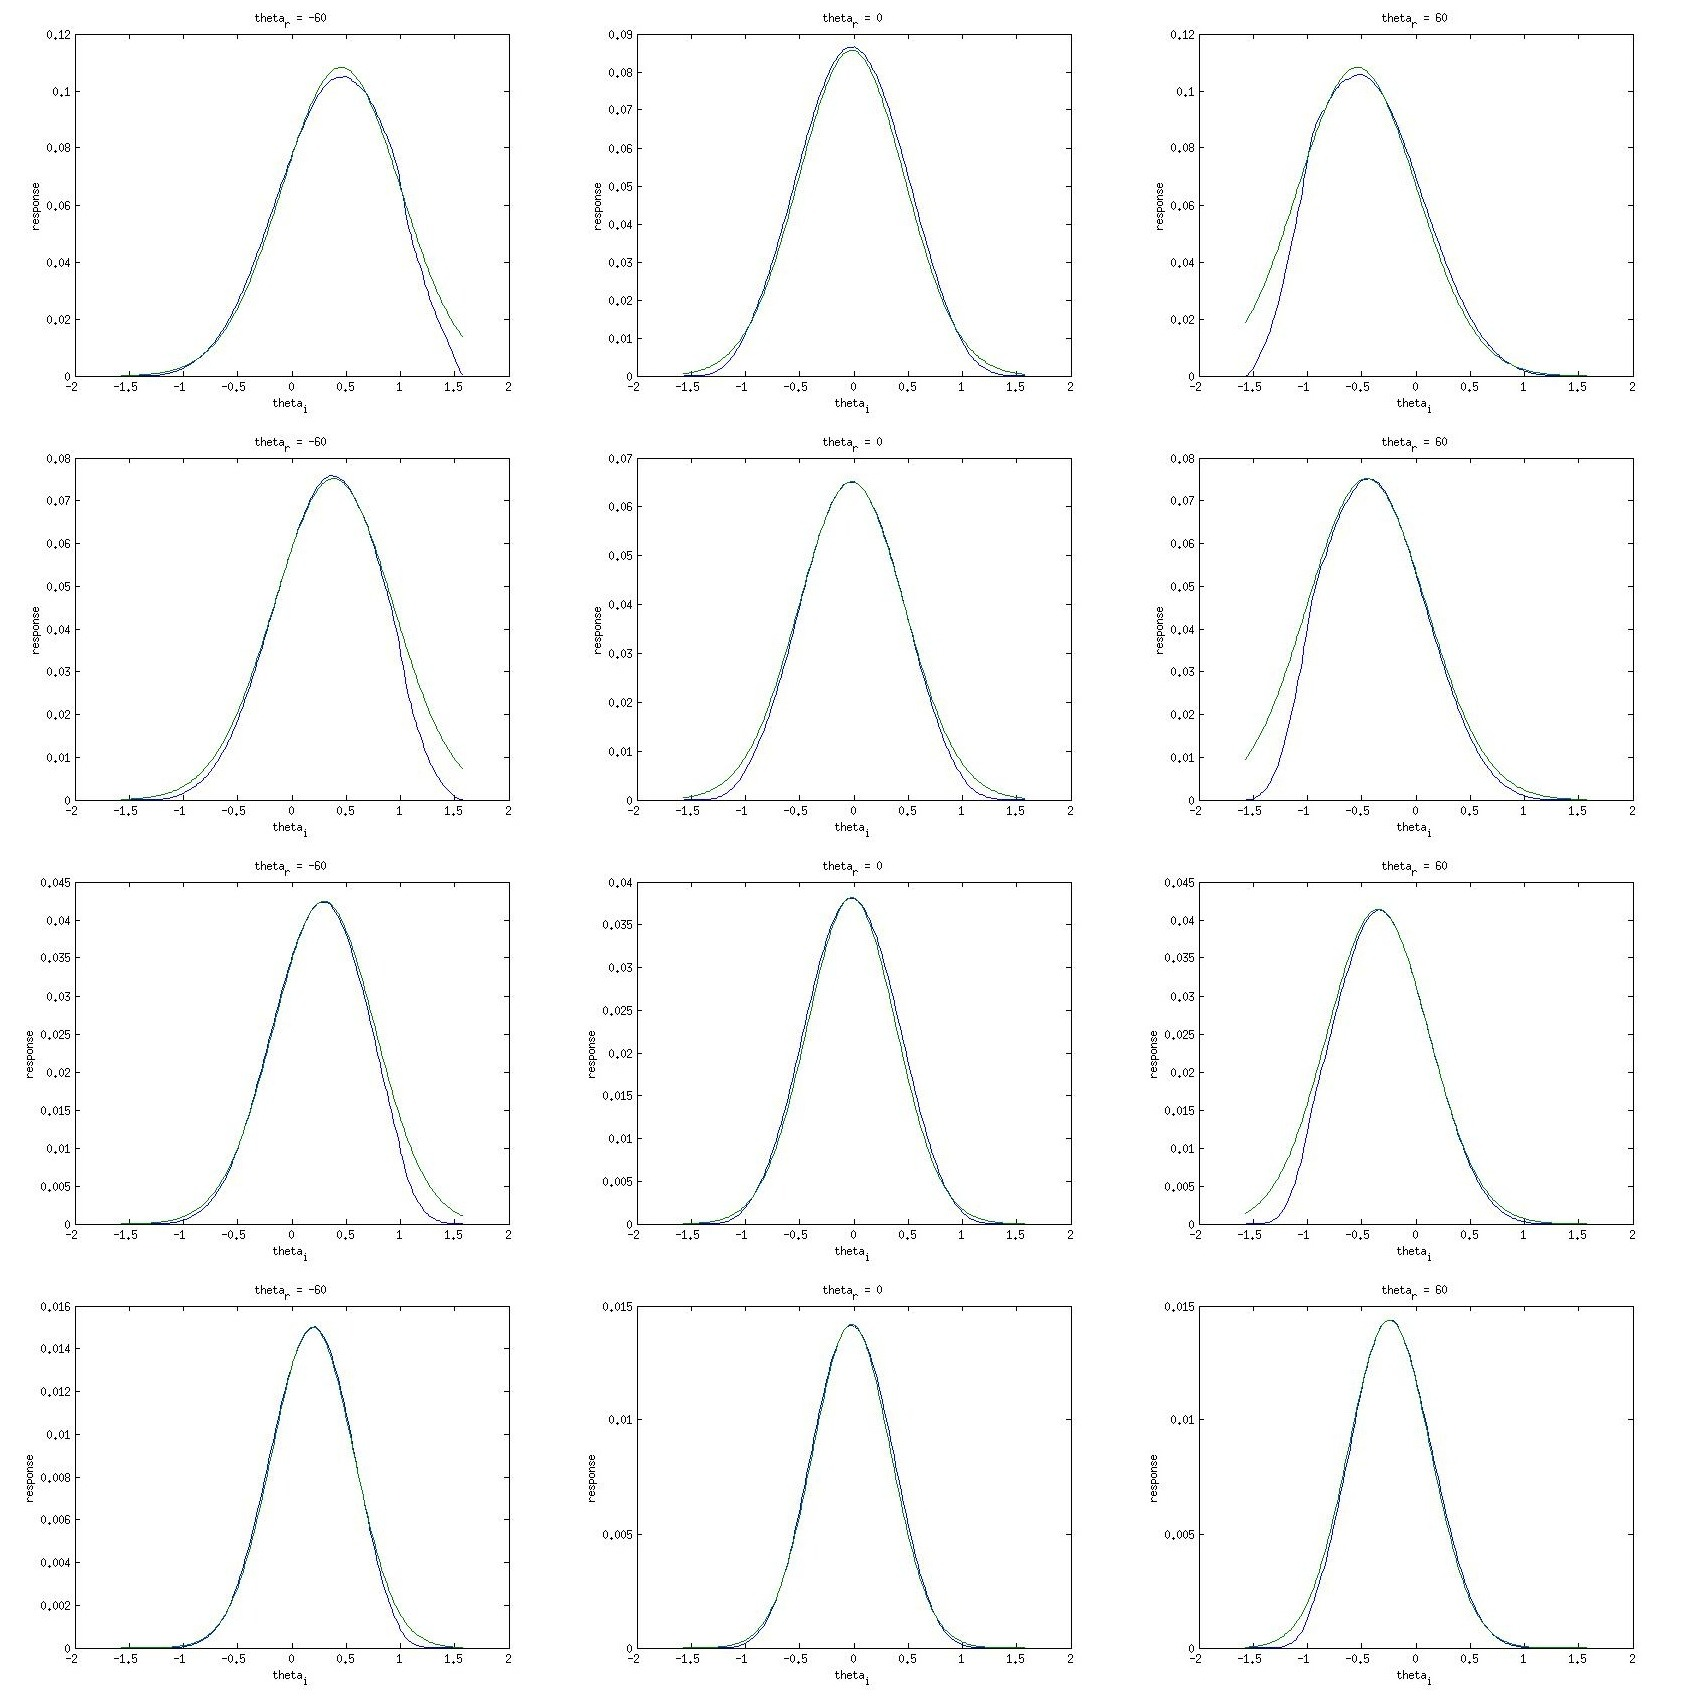
\includegraphics[scale=0.20]{images/graphfitting/fitting_combined.jpg}
\caption{A 2D slice of the scattering distribution for different number of hair strands that the light scatters through versus different $\theta_r$ (from left to right: -60, 0 and 60 degrees). The top row corresponds to 1, the second to 2, the third to 4 and the last row to 8 number of hair strands through which the light scatters. The scattering distribution is shown in blue and the generated gaussian function is green.}
\label{fitting}

\end{center}
\end{figure}

Figure~\ref{fitting} shows the fitting of the Gaussian functions for multiple scattering through 1, 2, 4 and 8 fibers. As can be seen is that the Gaussian functions match pretty well. As $\theta_r$ increases, the distribution becomes a bit distorted and deviates slightly from the generated gaussian function. We deliberately do not take this behaviour into account, although it is of course best to match the underlying distribution perfectly. In this case, it is a compromise between having an efficient function that matches the underlying PDF pretty well and is easy to integrate and evaluate, versus a complex function that is hard to integrate and expensive to evaluate. If the function becomes too expensive to evaluate, then uniform sampling might be more efficient after all.



\subsection{Comparing the scattering distribution with the generated distribution}
[TODO: show the effect of a generated distribution and compare it to the original distribution]


\end{document}